\documentclass[../main/main.tex]{subfiles}


\begin{document}

\section{March 17th, 2021}
\subsection{Moral Emotions}
\begin{description}
  \item[Sigmund Freud]
\begin{itemize}
\item Moral rules learned through identification with the same-sex parent during Phallic Stage
  \item Superego develops at age 5 or 6
        \begin{itemize}
\item Conscience - Disobedience leads to \vocab{guilt}.
          \item Ego ideal - Failure to live up to these standards brings shame
                \item Children obey conscience and ego ideal to avoid negative feelings i.e. moral emotions lead to moral behaviors.
        \end{itemize}
\item Freud believes that we should follow our superego.
\end{itemize}
        \item[Erikson]
        \begin{itemize}
          \item Children learn moral rules from both parents
                \item Besides guilt and shame, \vocab{pride} is just as important in moral development.
        \end{itemize}

\end{description}

\subsubsection{Research Support}
\begin{itemize}
\item Feelings of shame, guilt, and pride occurs at around age 6.
        \item The role of parents in forming moral emotions.
\end{itemize}
\subsubsection{Research Against}
\begin{itemize}
  \item Factors that determine guilt
\begin{description}
        \item[Cognitive Development]- Younger children feel guilty only when caught
  \item[Parenting Style] - Children of parents who use power-assertive discipline display less guilt
\end{description}
\end{itemize}

\subsection{Moral Reasoning}
\begin{definition}[Moral Reasoning]
The process of making judgments about the rightness or wrongness of specific acts.
\end{definition}

\subsubsection{Piaget’s Two-Stage Theory}
According to Piaget, moral judgment occurs during the concrete operational thinking (age 7-12).
\begin{description}
	\item[Moral Realism (Age < 8):]
        \begin{itemize}
          \item Rules are inflexible because they are set by authorities
          \item Rule violation would inevitably lead to punishment
          \item Strict obedience of rules
                \item Focus on outcomes rather than intention
        \end{itemize}
        \item[Moral Relativism (age $\geq$ 8):]
        \begin{itemize}
          \item Rules can be changed through social agreement.
          \item Punishment does not necessarily follows rule violations unless you get caught
            \item Moral judgments based on both intention and outcomes
          \item Intentional vs. unintentional act
                \item More weight is given to intentions than to outcomes
        \end{itemize}
\end{description}
\subsubsection{Kohlberg's Theory of Moral Reasoning}
Moral dilemma of stealing a drug to save his wife.\\

Kohlberg believes there are three levels of moral reasoning
\begin{description}
	\item[Preconvetional Reasoning:] Judgements are based on positive or negative consequences (external rewards and punishments) and authority figures

        \begin{itemize}
          \item Punishment and obedience orientation
          \item reward orientation
        \end{itemize}
        \begin{example}
\begin{itemize}
\item ``He should steal the drug for his wife because if she dies he'll have to pay for the funeral, and that costs a lot.''
        \item ``He should not steal the medicine because he would consequently be put in prison, which would mean he is a bad person''
\end{itemize}
        \end{example}
        \item[Conventional Reasoning:]Judgements are based on rules or norms of a group to which the indivudual belongs
        \begin{itemize}
          \item ``Good boy/nice girl stage'' - e.g. rewarded by parents.
          \item Authority and social-order-maintaining morality - we have to obey the society's rules
        \end{itemize}
        \begin{example}
\begin{itemize}
\item ``He should steal the medicine because his wife expects it; he wants to be a good husband.''
        \item ``He should not steal the medicine because the law prohibits stealing, making it illegal.''
\end{itemize}
        \end{example}
        \item[Postconventional Reasoning:]Judgements based on emergence of a personal reasoning. If the law is not fair, we must change it, and do not have to abide by it.
        \begin{itemize}
          \item Morality of contract, individual rights, and democratically accepted law, e.g. civil disobedience
          \item Morality of individual principles of conscience. Make moral decisions based on universal principles, e.g. basic respect and justice.
        \end{itemize}
        \begin{remark}
Laws change over time to reflect social values.
        \end{remark}
        \begin{example}
          ``Heshould steal the medicine, because saving a human life is a more fundamental value than the property rights of another person.''
        \end{example}
\end{description}
\begin{itemize}
  \item Kohlberg believe that the sequence is universal and invariant
        \item Not all individuals will progress through all 6 stages.
        \begin{remark}
Only a small amount of people are at stage 6.
        \end{remark}
        \item Research findings showed that there is a close relationship between the stage and age.
\end{itemize}
\begin{figure}[htpb]
	\centering
	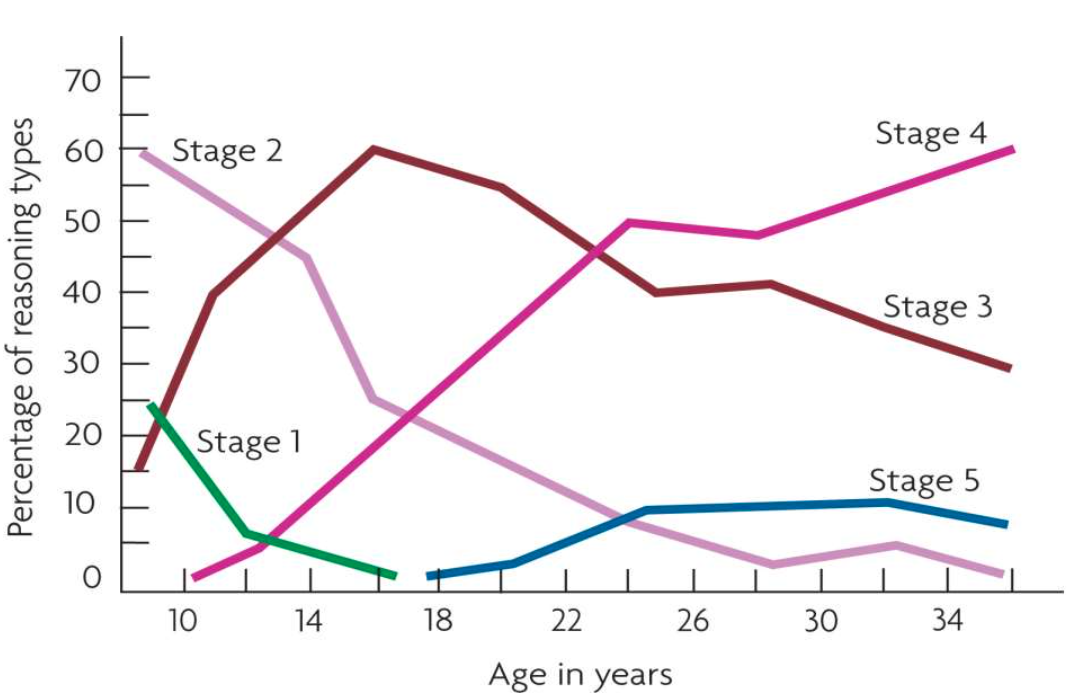
\includegraphics[width=0.8\textwidth]{../images/3-17-log}
	\caption{Study of Kohlberg's Theory of Moral Reasoning}
	\label{fig:}
\end{figure}
Factors that promote Moral Development
\begin{itemize}
\item Cognitive development is needed to progress from stage to stage (nature)
        \begin{itemize}
\item Decline of egocentrism is critical
                \item Perspective-taking improves an adolescent's ability to reason from another's perspective
        \end{itemize}
  \item Support from the social environment (nurture)
        \begin{itemize}
\item Opportunities for reciprocal dialogue about moral issues.
        \end{itemize}
\end{itemize}
\end{document}
